\chapter{Grundlagen}

\section{Grundlagen der Audio-DSP}

\subsection{Physikalische Grundlage des Audiosignals}

Das Audiosignal ist physikalisch eine sich in einem Medium ausbreitende Druck- und Bewegungsstörung, die durch ihre zeitlichen und räumlichen Schwingungsgrößen beschrieben wird.

Die einfachste Darstellung eines Signals im Zeitbereich ist die Sinuswelle,  

\begin{equation}
	x(t) = A \cdot \sin(\omega t + \phi)
\end{equation}
also eine zeitliche Schwankung des Drucks um einen Mittelwert \cite[Vgl.][S. ~504]{rossing2007springer}. 

Die wichtigsten Größen im Zeitbereich sind:

\begin{itemize}
	\item \textbf{Amplitude} $A$: die Größe der Schwingung, also die maximale Druckabweichung vom Ruhezustand.
	\item \textbf{Frequenz} $f$: die Anzahl der Schwingungswiederholungen pro Sekunde, gemessen in Hertz~(Hz).
	\item \textbf{Periode} $T$: die Dauer einer vollständigen Schwingung, mit
	\begin{equation}
		T = \frac{1}{f}
	\end{equation}
	\item \textbf{Phase} $\phi$: die Anfangslage der Schwingung im Zyklus, angegeben in Radiant.
\end{itemize}


\subsection{Abtastung und Quantisierung}
Abtastung auch als Sampling bezeichnet dient dazu aufgrund dessen, dass das analoge Signale zu jedem Zeitpunkt existiert, wird zu bestimmten, gleichmäßigen Zeitpunkten das Signal abgetastet, gemessen. Alles dazwischen wird ignoriert. Die Anzahl der Messungen pro Sekunde ist die Abtastfrequenz $f_s$ gemessen in Hz.

Bei der Abtastung ist die wichtigste Regel das $Nyquist-Theorem$. Sie besagt, dass mindestens doppelt so schnell abtasten wie die höchste Frequenz im Signal geben soll, sonst kommt es zu Fehlern. 
\begin{equation}
	f_s \geq 2 \cdot f_{\max}
\end{equation} \cite[Vgl.][S. ~521-522]{rossing2007springer}. 

Quantisierung ist der Schritt nach der Abtastung. Die unendlich genaue Messwerte werden auf einen diskreten Zahlenwert gerundet. Sie wird durch die Bittiefe begrenzt. Durch das Runden wird ein Quantisierungsfehler erzeugt, wobei ein leises Rauschen aus dem Differenz wahrgenommen wird. Je mehr Bits umso besser die Audioqualität \cite[Vgl.][S. ~520]{rossing2007springer}. 

\begin{equation}
	x[n] = x(n \cdot T_s), \quad T_s = \frac{1}{f_s}
\end{equation}

\subsection{Signal-Rausch-Verhältnis (SNR)}
SNR beschreibt das Verhältnis der Nutzleistung eines Signals zur Leistung des überlagerten 
Rauschens. Je höher das SNR, desto weniger wird das Nutzsignal durch Rauschen 
beeinträchtigt. \cite[Vgl.][S. ~5-6]{Loizou2013}

Das SNR ist definiert als:

\begin{equation}
	\text{SNR} = \frac{P_{\text{Signal}}}{P_{\text{Rauschen}}}
\end{equation}

Da Leistungsverhältnisse sehr große oder sehr kleine Zahlen annehmen können, 
wird das SNR in der Praxis logarithmisch in Dezibel (dB) angegeben:

\begin{equation}
	\text{SNR}_{\text{dB}} = 10 \cdot \log_{10} 
	\left( \frac{P_{\text{Signal}}}{P_{\text{Rauschen}}} \right)
\end{equation}

Sind statt Leistungen die Amplituden bekannt, gilt:

\begin{equation}
	\text{SNR}_{\text{dB}} = 20 \cdot \log_{10} 
	\left( \frac{A_{\text{Signal}}}{A_{\text{Rauschen}}} \right)
\end{equation}

Typische Orientierungswerte für die Sprachverarbeitung:

\begin{itemize}
	\item $\text{SNR} < 0\,\text{dB}$: Rauschen lauter als Nutzsignal
	\item $\text{SNR} \approx 10\,\text{dB}$: Sprache gerade noch verständlich
	\item $\text{SNR} \approx 20\,\text{dB}$: gute Sprachqualität
	\item $\text{SNR} > 40\,\text{dB}$: Studioqualität
\end{itemize}

Für die spektrale Subtraktion ist das SNR die zentrale Bewertungsgröße: 
Ziel des Algorithmus ist es, das SNR des verrauschten Eingangssignals 
$y[n] = x[n] + d[n]$ durch Unterdrückung des Rauschspektrums $D[k]$ 
zu maximieren, ohne dabei das Nutzsignal $x[n]$ wesentlich zu verzerren. \cite[S. ~23]{Loizou2013}

Für die spektrale Subtraktion ist das Signal-Rausch-Verhältnis besonders wichtig, weil das Verfahren darauf abzielt, den Rauschanteil im gestörten Sprachsignal zu verringern und damit die Verständlichkeit der Sprache zu verbessern. Die Qualität der Methode lässt sich deshalb wesentlich daran beurteilen, wie stark sich das Verhältnis zwischen Nutzsignal und Rauschen durch die spektrale Bearbeitung verbessert.

\subsection{Digitale Audiosignale als Sample-Folgen}

Nach Abtastung und Quantisierung liegt das Audiosignal als diskrete 
Sample-Folge vor:

\begin{equation}
	x[n] = x(n \cdot T_s), \quad n = 0, 1, \ldots, N-1
\end{equation}

Für die Verarbeitung wird die Folge in überlappende Frames der Länge 
$N$ unterteilt um den Verlust von Signalen zu vermeiden:

\begin{equation}
	x_\lambda[n] = x[n + \lambda \cdot H]
\end{equation}

\noindent wobei $\lambda$ den Frame-Index und $H$ die Hop Size bezeichnen. 
Diese blockbasierte Struktur ist die direkte Grundlage der 
Kurzzeit-Fouriertransformation in Abschnitt~\ref{sec:stft} 
\cite[Vgl.][S.~32-39]{Loizou2013}.

Für die spektrale Subtraktion ist diese Darstellung als diskrete Sample-Folge notwendig, weil das Signal nicht kontinuierlich, sondern blockweise verarbeitet wird. Erst durch die Zerlegung in kurze Frames kann später für jeden Zeitabschnitt ein separates Kurzzeitspektrum berechnet und bearbeitet werden.

\section{Frequenzanalyse mit DFT und FFT}
Die Frequenzanalyse ist eine zentrale Grundlage der digitalen Sprachsignalverarbeitung, weil sie ein Signal nicht nur als zeitlichen Verlauf, sondern auch als Zusammensetzung einzelner Frequenzanteile beschreibt.

\subsection{Zeitbereich und Frequenzbereich}

Im Zeitbereich wird ein digitales Signal als Amplitude über der Abtastzeit beziehungsweise über der Abtastnummer dargestellt. Diese Darstellung beschreibt also, wie sich der Signalwert im Verlauf der Zeit ändert. \cite[Vgl.][S.~91]{tan2018digital}

Im Frequenzbereich wird dasselbe Signal dagegen durch sein Spektrum beschrieben, also durch die Amplituden seiner enthaltenen Frequenzkomponenten. In dieser Darstellung liegt die Frequenz auf der x-Achse, in Hertz, während die y-Achse die Signalamplitude oder Spektralamplitude angibt.
\cite[Vgl.][S.~91]{tan2018digital}

Tan und Jiang zeigen diesen Zusammenhang bereits zu Beginn des Buches anhand einfacher Audiosignale: Ein 1000-Hz-Signal erscheint im Zeitbereich als periodische Schwingung, während im Frequenzbereich ein deutliches Maximum bei 1000 Hz sichtbar wird. Für ein Signal mit zwei Frequenzanteilen entstehen entsprechend zwei spektrale Peaks, etwa bei 1000 Hz und 3000 Hz. \cite[Vgl.][S.~4]{tan2018digital}

Der Wechsel in den Frequenzbereich ist notwendig, weil viele Verarbeitungsaufgaben dort leichter interpretierbar und effizienter durchführbar sind.

\begin{figure}[htbp]
	\centering
	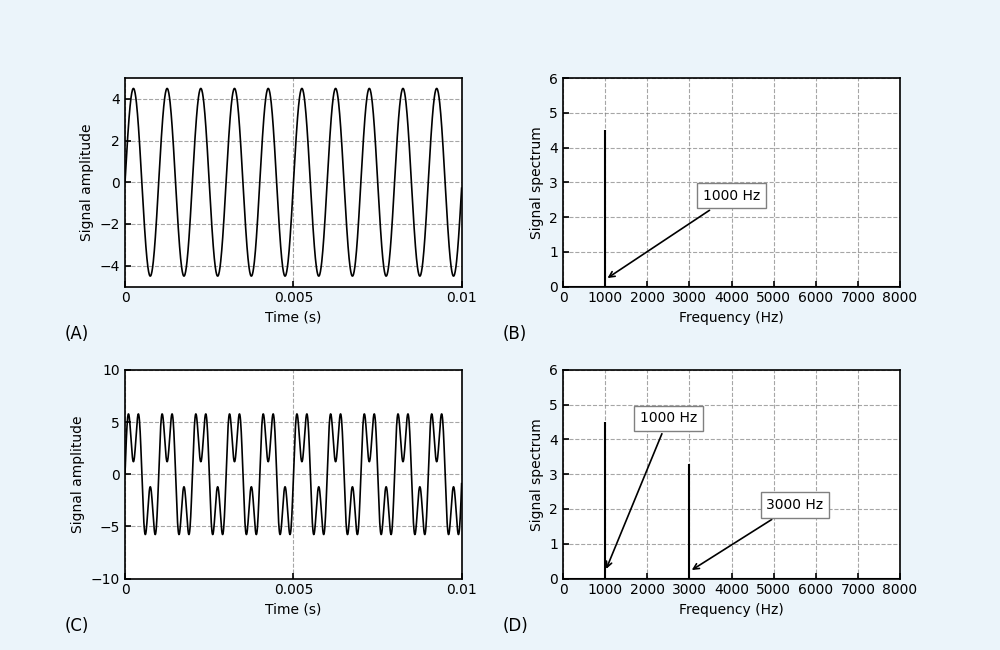
\includegraphics[width=0.8\textwidth]{images/time_frequency}
	\caption{Zeit- und Frequenzbereich Darstellung. Visualisierung generiert durch KI (Gemini, Version 3.1)}
	\label{fig:dsp_signals}
\end{figure}

Für die spektrale Subtraktion ist der Wechsel in den Frequenzbereich entscheidend, weil sich Sprache und Rauschen dort als spektrale Anteile beschreiben und voneinander trennen lassen. Das Verfahren arbeitet deshalb nicht direkt auf dem Zeitsignal, sondern auf den Frequenzkomponenten kurzer Sprachsegmente. \cite[Vgl.][S. 113-117]{boll1979}

\subsection{Diskrete Fourier-Transformation}

Die mathematische Grundlage für den Übergang vom Zeitbereich in den Frequenzbereich ist die diskrete Fourier-Transformation, kurz DFT. Sie ordnet einer endlichen Folge von Abtastwerten $x[n]$ ein Spektrum $X[k]$ zu, das die Frequenzanteile des Signals beschreibt. \cite[Vgl.][S.~91]{tan2018digital}

Die DFT ist definiert durch
\begin{equation}
	X[k] = \sum_{n=0}^{N-1} x[n] \cdot e^{-j 2\pi kn/N},
	\quad k = 0, 1, \ldots, N-1
\end{equation}
wobei $N$ die Anzahl der Signalwerte, $n$ den Zeitindex und $k$ den Frequenzindex bezeichnet. \cite[Vgl.][S.~97]{tan2018digital}

Der komplexe Exponentialterm kann auch in der Kurzschreibweise $W_N^{kn}$ mit dem Twiddle-Faktor $W_N$ geschrieben werden. \cite[Vgl.][S.~97]{tan2018digital}
Jeder DFT-Koeffizient $X[k]$ ist im Allgemeinen eine komplexe Zahl. Er beschreibt, wie stark die zum Index $k$ gehörende Frequenzkomponente im Signal vertreten ist und welche Phasenlage sie besitzt. \cite[Vgl.][S.~137]{tan2018digital}
Die inverse Transformation rekonstruiert aus dem Spektrum wieder das Zeitsignal. Tan und Jiang geben die inverse DFT in der Form
\begin{equation}
x[n] = \frac{1}{N} \sum_{k=0}^{N-1} X[k] \cdot W_N^{-kn}
\end{equation}
an und zeigen damit, dass DFT und inverse DFT ein Transformationspaar bilden. 
Ein praktischer Nachteil der direkten DFT ist ihr hoher Rechenaufwand. Für eine Folge der Länge $N$ ergibt sich bei direkter Berechnung eine Komplexität von $O(N^2)$.
\cite[Vgl.][S.~129]{tan2018digital}

Die DFT bildet damit die mathematische Grundlage der spektralen Subtraktion. Sie liefert für jedes Frame die Frequenzbins, in denen später der geschätzte Rauschanteil vom gestörten Sprachspektrum subtrahiert werden kann.

\subsection{Fast Fourier Transformation}

Da die direkte Berechnung der diskreten Fourier-Transformation (DFT) bei großen Signallängen mit einem hohen Rechenaufwand verbunden ist, wird in der Praxis die Fast Fourier Transformation (FFT) eingesetzt. Die FFT ist ein effizienter Algorithmus zur Berechnung der DFT-Koeffizienten und reduziert die Anzahl der erforderlichen komplexen Multiplikationen erheblich \cite[Vgl.][S. 127-130]{tan2018digital}.

Die Effizienz der FFT beruht darauf, dass die Berechnung der DFT nicht mehr unmittelbar aus ihrer Summendefinition erfolgt, sondern in kleinere Teilprobleme zerlegt wird. Tan und Jiang behandeln hierzu insbesondere radix-2-Algorithmen in den Varianten Decimation-in-Frequency und Decimation-in-Time. Dabei wird eine $N$-Punkt-DFT schrittweise in kleinere DFTs zerlegt, wodurch sich die Berechnung deutlich effizienter durchführen lässt \cite[Vgl.][S. 127--134]{tan2018digital}.

Für eine Datenlänge von $N$ benötigt die direkte DFT insgesamt $N^2$ komplexe Multiplikationen. Die FFT reduziert diesen Aufwand auf
\begin{equation}
	\frac{N}{2}\log_2 N
\end{equation}
komplexe Multiplikationen \cite[Vgl.][S. 129]{tan2018digital}.

Der theoretische Beschleunigungsfaktor der FFT gegenüber der direkten DFT ergibt sich damit zu
\begin{equation}
	\frac{N^2}{\frac{N}{2}\log_2 N}
	=
	\frac{2N}{\log_2 N}
\end{equation}

Für typische Signallängen zeigt sich daraus der in Tabelle~\ref{tab:fft-speedup} dargestellte Geschwindigkeitsvorteil.

\begin{table}[htbp]
	\centering
	\begin{tabular}{rrrr}
		\toprule
		$N$ & DFT ($N^2$) & FFT ($\frac{N}{2}\log_2 N$) & Speedup \\
		\midrule
		256  & 65{,}536     & 1{,}024   & 64$\times$ \\
		1024 & 1{,}048{,}576 & 5{,}120   & 205$\times$ \\
		4096 & 16{,}777{,}216 & 24{,}576 & 683$\times$ \\
		\bottomrule
	\end{tabular}
	\caption{Vergleich des theoretischen Rechenaufwands von DFT und FFT}
	\label{tab:fft-speedup}
\end{table}

Ein anschauliches Beispiel geben Tan und Jiang für eine Folge mit 1024 Datenpunkten. Für die direkte DFT werden dabei 1{,}048{,}576 komplexe Multiplikationen benötigt, während die FFT nur 5{,}120 komplexe Multiplikationen erfordert \cite[Vgl.][S. 130]{tan2018digital}. Damit wird die praktische Relevanz der FFT insbesondere für große Datenmengen und Echtzeitanwendungen deutlich.

Für die praktische Implementierung der spektralen Subtraktion ist nicht nur die DFT, sondern vor allem die FFT wichtig, weil sie die spektrale Analyse und die spätere inverse Transformation rechnerisch effizient macht. Gerade für framebasierte Sprachverarbeitung und Echtzeitanwendungen ist diese Beschleunigung entscheidend.

\subsection{Amplituden- und Leistungsspektrum}

Die DFT liefert für jedes Frequenzbin einen komplexen Koeffizienten $X(k)$. Da komplexe DFT-Koeffizienten nicht direkt anschaulich dargestellt werden können, werden in der Praxis daraus Betrag und Phase bestimmt. Der Betrag bildet dabei die Grundlage für das Amplitudenspektrum, während das Quadrat des Betrags zur Berechnung des Leistungsspektrums verwendet wird \cite[Vgl.][S. 103]{tan2018digital}.

Das Amplitudenspektrum ist definiert als
\begin{equation}
	A_k = \frac{1}{N}\left|X(k)\right|
	= \frac{1}{N}\sqrt{\left(\operatorname{Re}\{X(k)\}\right)^2 + \left(\operatorname{Im}\{X(k)\}\right)^2},
	\quad k = 0,1,2,\ldots,N-1
\end{equation}

Das Leistungsspektrum ergibt sich entsprechend zu
\begin{equation}
	P_k = \frac{1}{N^2}\left|X(k)\right|^2
	= \frac{1}{N^2}\left[\left(\operatorname{Re}\{X(k)\}\right)^2 + \left(\operatorname{Im}\{X(k)\}\right)^2\right],
	\quad k = 0,1,2,\ldots,N-1
\end{equation}

In vielen praktischen Anwendungen wird statt des zweiseitigen Spektrums ein einseitiges Spektrum betrachtet. Dabei bleibt der Gleichanteil bei $k=0$ unverändert, während die übrigen Spektralanteile bis zur Faltungsfrequenz verdoppelt werden. Tan und Jiang geben für das einseitige Amplitudenspektrum die Form
\begin{equation}
	A_k =
	\begin{cases}
		\frac{1}{N}\left|X(0)\right|, & k = 0 \\[6pt]
		\frac{2}{N}\left|X(k)\right|, & k = 1,\ldots,\frac{N}{2}
	\end{cases}
\end{equation}
an \cite[Vgl.][S. 103]{tan2018digital}.

Die graphische Darstellung von Amplituden- und Leistungsspektrum zeigt, wie sich die Energie eines Signals auf einzelne Frequenzen verteilt. Tan und Jiang veranschaulichen dies sowohl für DFT als auch für FFT anhand von Spektralplots, in denen charakteristische Peaks an den dominanten Frequenzkomponenten sichtbar werden \cite[Vgl.][S. 109--110]{tan2018digital}.

Für die spektrale Subtraktion ist besonders das Amplituden- beziehungsweise Magnitudenspektrum relevant, weil im klassischen Verfahren nach Boll der geschätzte Rauschbetrag direkt vom Betrag des gestörten Sprachspektrums abgezogen wird. Das Spektrum ist damit die eigentliche Arbeitsdarstellung des Verfahrens.

\subsection{Frequenzauflösung}

Ein zentraler Parameter der Spektralanalyse ist die Frequenzauflösung. Sie beschreibt den Frequenzabstand zwischen zwei benachbarten DFT-Koeffizienten und gibt damit an, wie fein das Spektrum im Frequenzbereich aufgelöst ist \cite[Vgl.][S. 101, 103]{tan2018digital}.

Die Frequenzauflösung ergibt sich zu
\begin{equation}
	\Delta f = \frac{f_s}{N}
\end{equation}
wobei $f_s$ die Abtastfrequenz und $N$ die Anzahl der ausgewerteten Datenpunkte bezeichnet \cite[Vgl.][S. 103]{tan2018digital}.

Aus dieser Beziehung folgt, dass eine größere Datenlänge $N$ zu einer besseren Frequenzauflösung führt. Tan und Jiang weisen ausdrücklich darauf hin, dass mit einer längeren Datenfolge eine feinere Auflösung im Frequenzbereich erreicht werden kann \cite[Vgl.][S. 103]{tan2018digital}. Eine größere Anzahl an Datenpunkten bedeutet zugleich, dass ein längerer Signalabschnitt ausgewertet werden muss. In der Spektralanalyse wird dazu eine Beobachtungsdauer von
\begin{equation}
	T_0 = NT
\end{equation}
verwendet, wobei $T = 1/f_s$ die Abtastperiode ist. Damit verbessert eine größere Fensterlänge zwar die Frequenzauflösung, erhöht aber gleichzeitig die Länge des ausgewerteten Zeitabschnitts \cite[Vgl.][S. 102]{tan2018digital}.

Die Frequenzauflösung bestimmt, wie fein Sprache und Rauschen im Spektrum voneinander getrennt werden können. Für die spektrale Subtraktion ist sie deshalb wichtig, weil eine zu grobe Auflösung die präzise Schätzung und Subtraktion des Rauschanteils in einzelnen Frequenzbereichen erschwert.

\section{Kurzzeitanalyse von Sprachsignalen}
Die Sprachsignalverarbeitung kann nicht allein auf einer globalen Fourier-Analyse über das gesamte Signal beruhen, da Sprachsignale zeitlich stark variieren. Für Verfahren wie die spektrale Subtraktion ist deshalb eine Kurzzeitanalyse erforderlich, bei der Sprache in kurze, überlappte Abschnitte zerlegt und für jedes Zeitfenster separat im Frequenzbereich beschrieben wird. \cite[Vgl.][S. 114, 116, 117]{boll1979} 
\subsection{Nichtstationarität von Sprache}
Sprachsignale sind im Allgemeinen nichtstationär, da sich ihre spektralen und zeitlichen Eigenschaften fortlaufend ändern. Boll weist ausdrücklich darauf hin, dass Sprache nichtstationär ist und deshalb nur eine begrenzte zeitliche Mittelung erlaubt ist. \cite[Vgl.][S. 114]{boll1979} 

Diese Eigenschaft ist für die Analyse entscheidend, weil eine zu lange Mittelung oder eine zu große Auswertezeit zu einer Verschmierung kurzer Sprachereignisse führen kann. \cite[Vgl.][S. 114, 116]{boll1979} 

Für die spektrale Subtraktion ist die Nichtstationarität von Sprache der Grund, warum nicht das Gesamtsignal auf einmal, sondern nur kurze Abschnitte analysiert werden. Innerhalb solcher kurzen Zeitfenster kann das Signal näherungsweise lokal stationär behandelt werden, was die spektrale Bearbeitung erst praktikabel macht.  \cite[Vgl.][S. 113, 114]{boll1979}

\subsection{Frame-basierte Verarbeitung}

Um Sprache kurzzeitig analysieren zu können, wird das Signal in einzelne Frames zerlegt. Boll beschreibt dieses Vorgehen konkret so, dass die Eingangsdaten in halb überlappte Datenpuffer segmentiert und anschließend mit einer Hanning-Funktion gewichtet werden. \cite[Vgl.][S. 116]{boll1979}

Für die saubere Rekonstruktion des Signals, verweist Boll darauf, dass bei halb überlappten Puffern und Hanning-Fensterung die summierten Fenster im Optimalfall wieder das ursprüngliche Signal. \cite[Vgl.][S. 116]{boll1979}

Zu beachten sind die Framelänge, die Schrittweite zwischen zwei Frames und die verwendete Fensterfunktion. Im Boll-Verfahren wird bei $f_s = 8\, \mathrm{kHz}$ eine Fensterlänge von 256 Punkten und eine Verschiebung um 128 Punkte verwendet, also eine Überlappung von 50\%. \cite[Vgl.][S. 116]{boll1979}

\subsection{Short-Time Fourier Transform}
\label{sec:stft}

Die Short-Time Fourier Transform, kurz STFT, beschreibt ein Signal nicht mehr nur global im Frequenzbereich, sondern als zeitabhängige Folge lokaler Spektren. Praktisch wird dazu auf jedes gefensterte Frame eine Fourier-Transformation angewendet, sodass für jedes Zeitfenster ein eigenes Kurzzeitspektrum entsteht. Diese Art der Analyse entspricht genau dem Vorgehen, das Boll für die spektrale Subtraktion beschreibt: Für jedes Datenfenster wird die DFT berechnet und daraus das Magnitudenspektrum bestimmt. \cite[Vgl.][S. 116]{boll1979}

Boll verwendet die kurzzeitigen Spektren direkt zur Darstellung von Zeit-Frequenz-Verläufen. Er beschreibt isometrische Darstellungen von Zeit gegen Frequenz und Spektralmagnitude, die aus 64 überlappten Hanning-Fenstern berechnet wurden; Als Ergebnis erhält man eine zeitlich vorlaufendes Spektrum statt einer einzigen globalen Fourier-Darstellung. \cite[Vgl.][S. 117]{boll1979}

\subsection{Magnitude und Phase}
Das Fourier-Spektrum kann in Betrag und Phase zerlegt werden. Wobei der Betrag das Amplitudenspektrum und deren Winkel das Phasenspektrum abbildet. 
Tan definiert das Amplitudenspektrum über den Betrag der komplexen DFT-Koeffizienten und das Phasenspektrum über deren Winkel. \cite[Vgl.][S. 103]{tan2018digital} Für die Sprachverarbeitung bedeutet das, dass jeder Frame nicht nur eine Verteilung von Beträgen über der Frequenz besitzt, sondern zusätzlich Phaseninformationen enthält.

Für die spektrale Subtraktion ist insbesondere die Magnitude entscheidend, weil im klassischen Verfahren der geschätzte Rauschbetrag vom Magnitudenspektrum des gestörten Signals abgezogen wird. Die Phase des Eingangssignals bleibt dagegen meist erhalten und wird erst bei der Rekonstruktion des Zeitsignals wieder verwendet.

\section{Theorie der Spectral Subtraction}
Wie in den vorherigen Unterkapiteln schon oft angesprochen wurde ist die Spektrale Subtraktion ein Verfahren zur Rauschminderung in Sprachsignalen. Die Grundidee besteht darin, den geschätzten Rauschanteil im Frequenzbereich vom gestörten Sprachsignal abzuziehen, um die Sprache klarer und verständlicher zu machen. \cite[Vgl.][S.113]{boll1979}.

Im Folgenden wird die Grundidee, das Signalmodell, die Verarbeitung im Frequenzbereich sowie die wichtigsten Voraussetzungen und Grenzen erklärt.
\subsection{Ziel und Grundidee des Verfahrens}
Ziel der Spectral Subtraction ist es, den Rauschanteil in einem Sprachsignal zu verringern und dadurch die Qualität der Sprache zu verbessern. Dazu wird zunächst das Rauschspektrum geschätzt und anschließend vom Spektrum des gestörten Signals subtrahiert. \cite[Vgl.][S.113-114]{boll1979}. 

\begin{figure}[htbp]
	\centering
	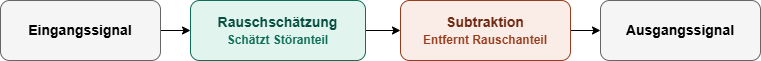
\includegraphics[width=0.8\textwidth]{images/rauschunterdrueckung}
	\caption{Blockdiagramm Spectral Subtraction, Visualisierung generiert durch KI (Gemini, Version 3.1)}
	\label{fig:spectral_subtraction}
\end{figure}

\subsection{Additives Modell von Sprache und Rauschen}
Die Methode basiert auf der Annahme, dass das beobachtete Signal aus Sprache und Rauschen zusammengesetzt ist. Im Zeitbereich gilt: 
\begin{equation}
	x(k)=s(k)+n(k)
\end{equation} 
\noindent \textbf{Variablen:}
\begin{itemize}
	\item x(k): beobachtetes, verrauschtes Signal im betrachteten Fenster
	\item s(k): sauberes Sprachsignal
	\item n(k): Rauschsignal
	\item k: Abtastindex innerhalb des betrachteten Fensters
\end{itemize}
Nach der Fourier-Transformation ergibt sich:

\begin{equation}
	X(e^{j\omega}) = S(e^{j\omega}) + N(e^{j\omega})
\end{equation}

\noindent \textbf{Variablen:}
\begin{itemize}
	\item $X(e^{j\omega})$: Spektrum des verrauschten Signals
	\item $S(e^{j\omega})$: Spektrum der sauberen Sprache
	\item $N(e^{j\omega})$: Spektrum des Rauschens
	\item $e^{j\omega}$: komplexe Darstellung einer Frequenzkomponente
	\item $\omega$: Kreisfrequenz
\end{itemize}
Im Frequenzbereich gilt dieselbe Idee, dort setzt sich das gestörte Spektrum aus Sprachspektrum und Rauschspektrum zusammen. \cite[Vgl.][S.114]{boll1979}.


\begin{figure}[htbp]
	\centering
	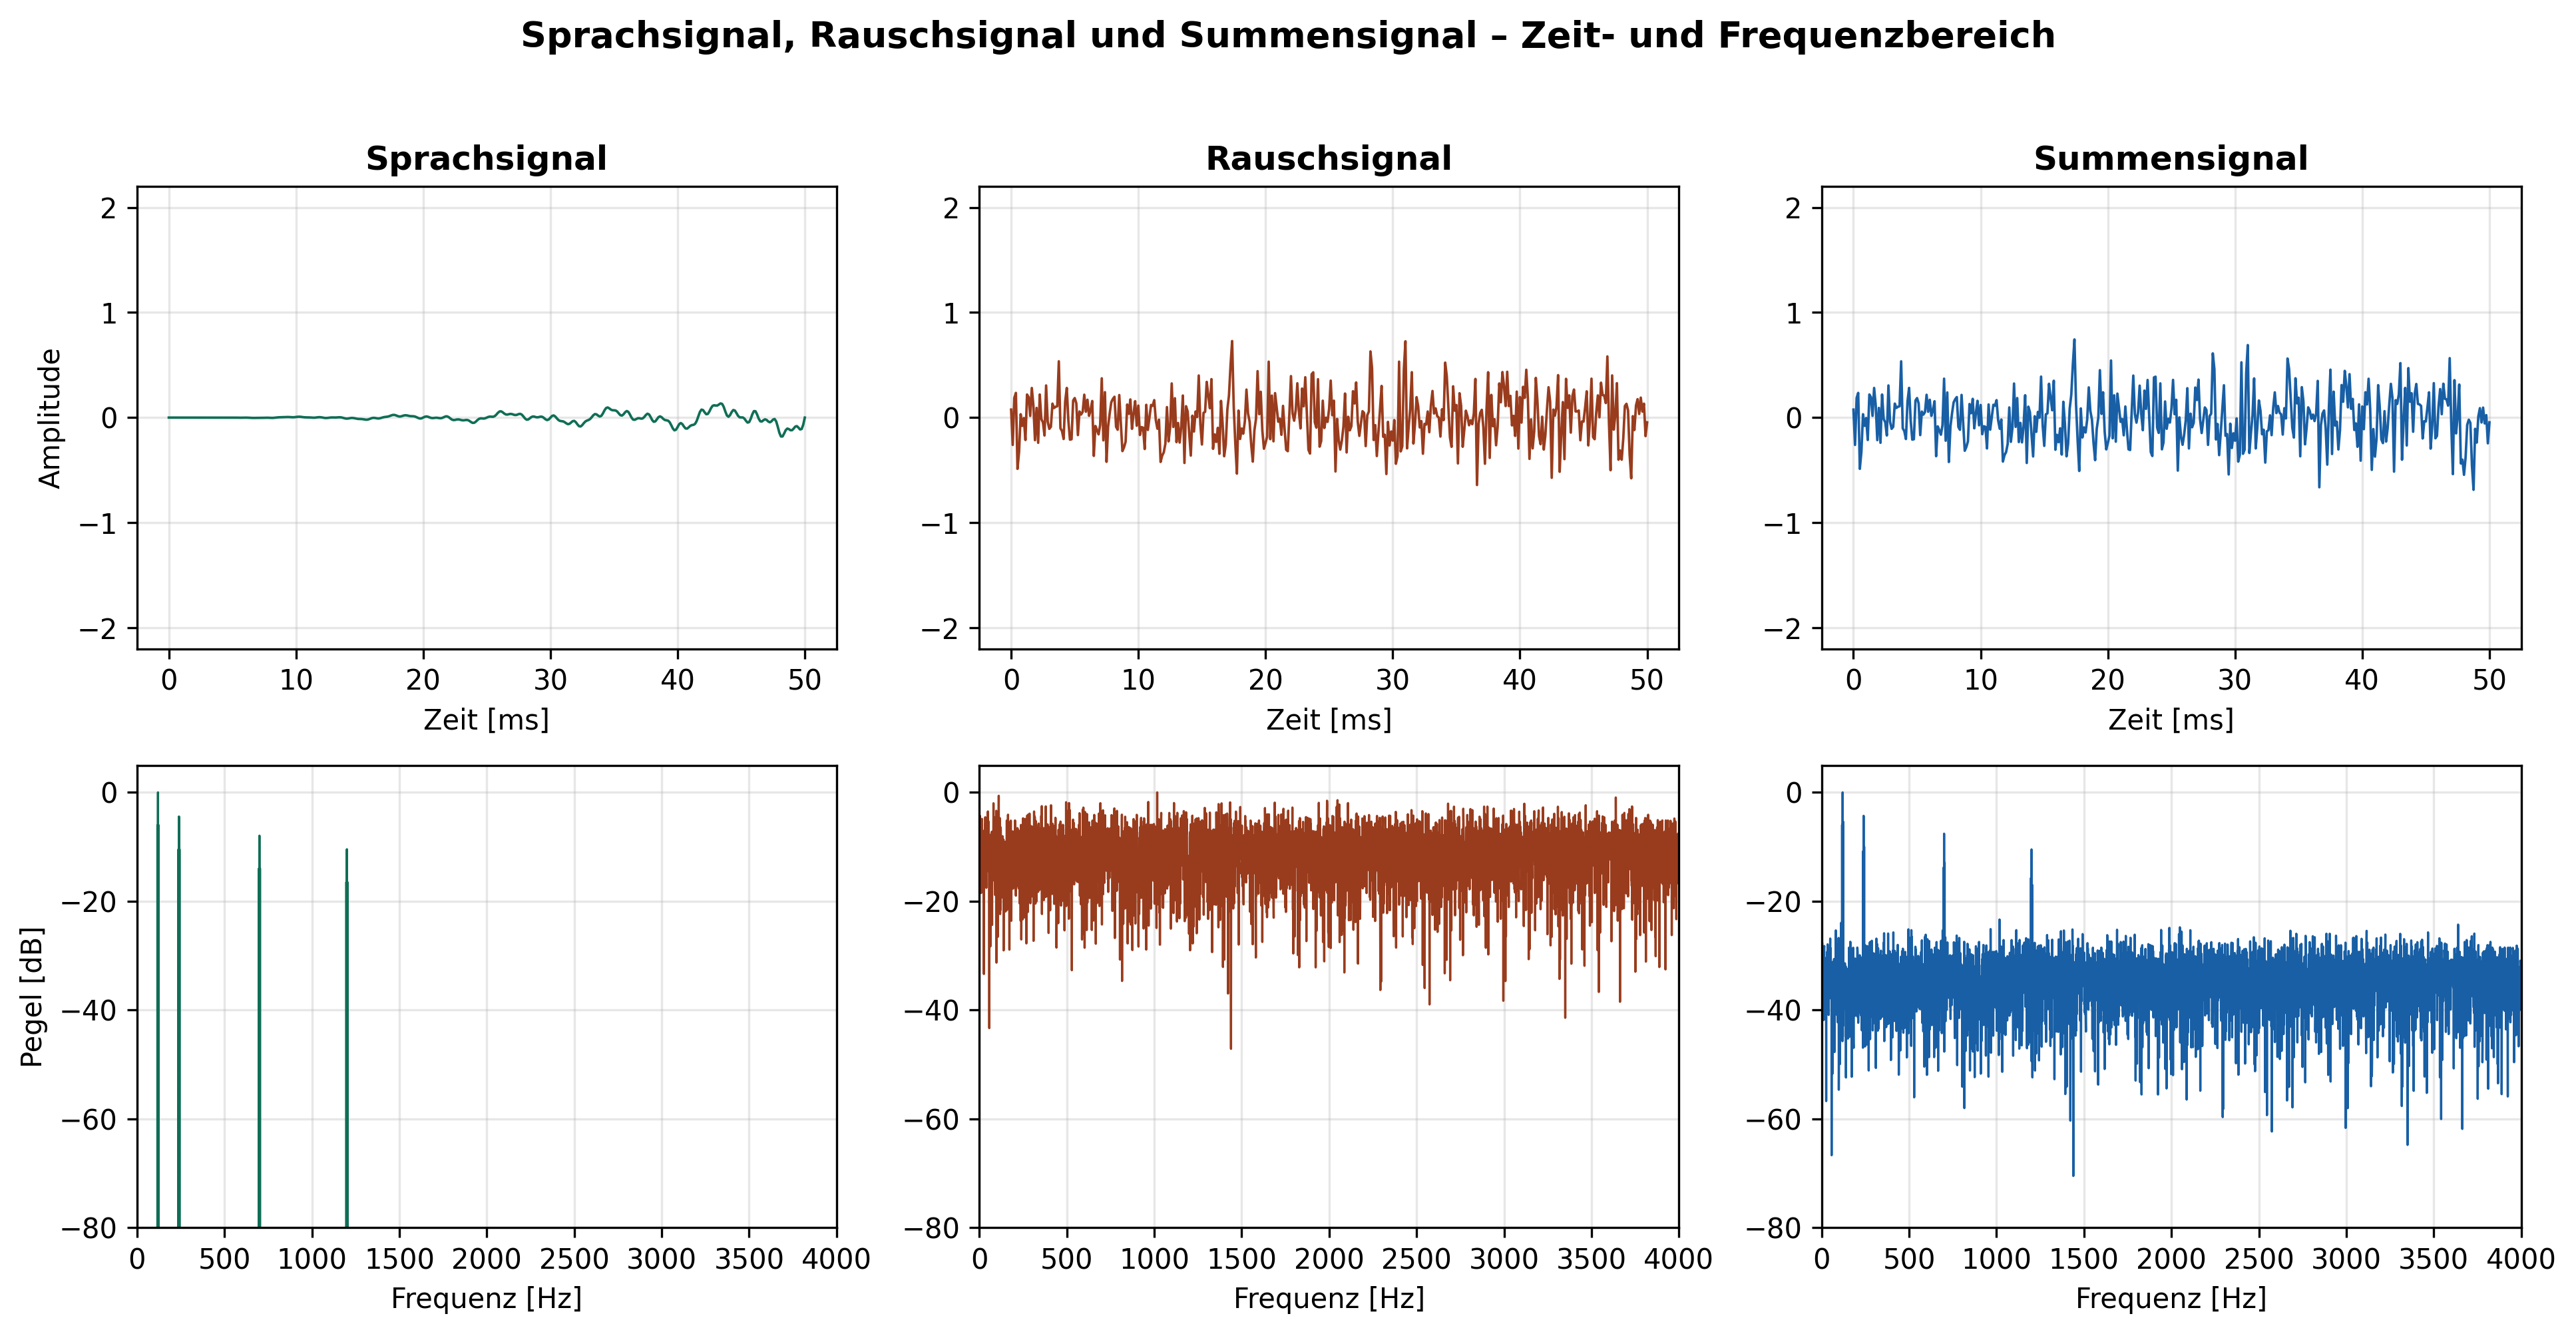
\includegraphics[width=0.8\textwidth]{images/summensignal.png}
	\caption{Sprachsignal, Rauschsignal und Summensignal im Zeit- und Frequenzbereich}
	\label{fig:signal-zeit-frequenz}
\end{figure}



\subsection{Grundablauf der Spectral Subtraction}
Der Ablauf der Spectral Subtraction lässt sich in wenige Schritte gliedern. Zuerst wird das Sprachsignal in kurze, meist überlappende Frames aufgeteilt und für jedes Frame in den Frequenzbereich transformiert.

Danach wird aus sprachfreien Abschnitten ein mittleres Rauschspektrum geschätzt
Im nächsten Schritt wird dieses geschätzte Rauschspektrum vom Magnitudenspektrum des gestörten Signals abgezogen. Wenn dabei negative Werte entstehen, werden sie auf null gesetzt. Dieser Schritt wird als Half-Wave Rectification bezeichnet. Er verhindert, dass nicht sinnvolle negative Spektralwerte weiterverarbeitet werden.

Anschließend können zusätzliche Verfahren zur Verringerung des verbleibenden Restrauschens eingesetzt werden. Zum Schluss wird aus dem bearbeiteten Spektrum wieder ein Zeitsignal rekonstruiert. Dazu wird die inverse Transformation verwendet und die einzelnen Frames werden per Overlap-Add zusammengesetzt. 
\cite[Vgl.][S.113-118]{boll1979}

\noindent \textbf{In vereinfachter Form besteht das Verfahren aus:}
\begin{enumerate}
	\item Segmentierung des Signals 
	\item Transformation in den Frequenzbereich
	\item Schätzung des Rauschspektrums
	\item spektrale Subtraktion
	\item Begrenzung negativer Werte
	\item optionale Restrauschminderung
	\item Rücktransformation und Rekonstruktion
\end{enumerate}
	
\begin{figure}[htbp]
	\centering
	\begin{tikzpicture}[
		% --- Definition der Block-Designs ---
		block/.style={
			rectangle, 
			draw=black!80, 
			thick, 
			fill=blue!5, 
			text width=5cm, 
			align=center, 
			minimum height=1.2cm, 
			font=\sffamily,
			rounded corners=1mm
		},
		io/.style={
			rectangle, 
			draw=black!80, 
			thick, 
			fill=gray!15, 
			text width=5cm, 
			align=center, 
			minimum height=1.2cm, 
			font=\sffamily\bfseries,
			rounded corners=4mm % Stärkere Rundung für Start/Ende
		},
		arrow/.style={
			->, 
			>=stealth, 
			thick,
			draw=black!80
		}
		]
		
		% --- Platzierung der Blöcke ---
		\node[io]    (in)       {Eingangssignal};
		\node[block] (framing)  [below=0.6cm of in]      {Framing und Fensterung};
		\node[block] (fft)      [below=0.6cm of framing] {FFT};
		\node[block] (sub)      [below=1.5cm of fft]     {Subtraktion};
		
		% Rauschschätzung wird rechts neben der Subtraktion platziert
		\node[block] (noise)    [right=1cm of sub]       {Rauschschätzung};
		
		\node[block] (hwr)      [below=0.6cm of sub]     {Half-Wave Rectification};
		\node[block] (ifft)     [below=0.6cm of hwr]     {IFFT};
		\node[block] (ola)      [below=0.6cm of ifft]    {Overlap-Add};
		\node[io]    (out)      [below=0.6cm of ola]     {Ausgangssignal};
		
		% --- Verbindungen (Pfeile) ziehen ---
		\draw[arrow] (in) -- (framing);
		\draw[arrow] (framing) -- (fft);
		\draw[arrow] (fft) -- (sub);
		\draw[arrow] (sub) -- (hwr);
		\draw[arrow] (hwr) -- (ifft);
		\draw[arrow] (ifft) -- (ola);
		\draw[arrow] (ola) -- (out);
		
		% Pfade für die Rauschschätzung
		% Pfeil von FFT (Osten) mit Knick nach unten zur Rauschschätzung (Norden)
		\draw[arrow] (fft.east) -| (noise.north);
		% Pfeil von Rauschschätzung (Westen) zur Subtraktion (Osten)
		\draw[arrow] (noise.west) -- (sub.east);
		
	\end{tikzpicture}
	\caption{Ablaufdiagramm der Signalverarbeitung zur Rauschunterdrückung}
	\label{fig:ablauf_spectral_subtraction}
\end{figure}

\subsection{Vorraussetzungen}

Die Spectral Subtraction funktioniert nicht unter allen Bedingungen gleich gut. Eine wichtige Voraussetzung ist, dass das Hintergrundrauschen wenigstens für kurze Zeit annähernd stationär bleibt. Wenn sich das Rauschen zu schnell ändert, wird die vorherige Rauschschätzung ungenau und die Subtraktion kann unwirksam oder sogar schädlich werden \cite[Vgl.][S.116]{boll1979}. 
 
Eine weitere Voraussetzung ist, dass sprachfreie Abschnitte erkannt werden können. Nur dann kann das Rauschspektrum zuverlässig neu geschätzt werden \cite[Vgl.][S.116-117]{boll1979}.

Außerdem kann es passieren, dass bei der Subtraktion auch schwache Sprachanteile entfernt werden. Das ist insbesondere dann problematisch, wenn an einer Frequenz die Summe aus Sprache und lokalem Rauschen kleiner ist als der geschätzte Rauschwert \cite[Vgl.][S.116-117]{boll1979}. In diesem Fall wird nicht nur Rauschen, sondern auch nützliche Sprachinformation unterdrückt. Es besteht also immer ein Kompromiss zwischen stabiler Rauschschätzung und guter zeitlicher Auflösung.

Trotz dieser Grenzen zeigt Boll, dass das Verfahren die Sprachqualität verbessern kann und in bestimmten Anwendungen auch die Verständlichkeit erhöht \cite[Vgl.][S.119]{boll1979} Die Methode ist deshalb theoretisch einfach, praktisch nützlich, aber stark von den Eigenschaften des Rauschens und von einer guten Parametrierung abhängig.
\section{Fensterung und spektrale Eigenschaften}

\subsection{Blockbildung und Randdiskontinuitäten}
Für die Kurzzeitanalyse wird das Sprachsignal nicht auf einmal transformiert, sondern zunächst in einzelne, endlich lange Blöcke unterteilt. Diese Zerlegung ist erforderlich, da Verfahren wie die spektrale Subtraktion auf kurzzeitigen Spektren basieren und das Signal daher frameweise verarbeitet werden muss. 
Boll beschreibt genau dieses Vorgehen, indem das Sprachsignal aus halb überlappenden Eingangspuffern analysiert wird. \cite[Vgl.][S. 114]{boll1979}

Ohne passende Gewichtung entstehen an den Blockrändern häufig Amplitudensprünge. Tan und Jiang erklären, dass diese Randdiskontinuitäten im Zeitbereich die Ursache für spektrale Verzerrungen im Frequenzbereich sind. \cite[Vgl.][S. 112]{tan2018digital}

Für die spektrale Subtraktion ist die Blockbildung unvermeidbar, weil das Verfahren auf kurzzeitigen Spektren basiert. Gleichzeitig muss verhindert werden, dass künstliche Randdiskontinuitäten das Spektrum verfälschen und dadurch die spätere Rauschschätzung oder Subtraktion ungenau wird. 

\subsection{Spectral Leakage}

Wie bereits erwähnt wird das Phänomen durch den Randdiskontinuitäten im Zeitbereich, als Spectral Leakage bezeichnet. Tan und Jiang zeigen, dass dabei im Spektrum zusätzliche Frequenzanteile erscheinen, die im ursprünglichen Signal nicht vorhanden sind. Die Ursache liegt in der zeitlichen Amplitudendiskontinuität des betrachteten Signalblocks. \cite[Vgl.][S. 112]{tan2018digital} Sie ist für die spektrale Subtraktion problematisch, weil Energie aus einem Frequenzbereich in benachbarte Bins verschmiert werden kann. Dadurch wird die binweise Subtraktion des geschätzten Rauschanteils ungenauer und es kann leichter zu Verzerrungen der Sprache kommen. \cite[Vgl.][S.113-117]{boll1979} Zur Verringerung dieses Effekts wird eine Fensterfunktion verwendet, deren Amplitude an beiden Enden glatt gegen Null ausläuft. Dadurch wird der Übergang zwischen den Blockrändern weicher, und die spektrale Leckage wird deutlich reduziert. \cite[Vgl.][S.113-117]{boll1979} \cite[Vgl.][S. 112]{tan2018digital}


\subsection{Hanning- und Hamming-Fenster}
Zu den gebräuchlichsten Fensterfunktionen gehören das Hanning- und das Hamming-Fenster. Tan und Jiang geben sie in der Form

\begin{equation}
	w_{hm}(n) = 0.54 - 0.46 \cos\left(\frac{2\pi n}{N-1}\right)
\end{equation}

und

\begin{equation}
	w_{hn}(n) = 0.5 - 0.5 \cos\left(\frac{2\pi n}{N-1}\right)
\end{equation}

an \cite[Vgl.][S. 115]{tan2018digital}.

Dabei gilt jeweils $0 \leq n \leq N-1$ , wobei $N$ die Fensterlänge (Anzahl der Samples) ist. Beide Fenster verringern die Amplitude an den Blockrändern und reduzieren dadurch die spektrale Leckage. \cite[Vgl.][S. 112]{tan2018digital}.

Für die spektrale Subtraktion ist diese Fensterwahl aus zwei Gründen zentral. Erstens verbessert sie die Qualität des geschätzten Kurzzeitspektrums vor der Subtraktion. Zweitens ermöglicht sie zusammen mit der 50\%-Überlappung eine saubere Resynthese des bearbeiteten Signals. \cite[Vgl.][S. 116,117]{boll1979}
  
\section{Verarbeitungsschritte der Spectral Subtraction} 
\subsection{Rauschschätzung in sprachfreien Abschnitten}
Die Spectral Subtraction benötigt zunächst eine Schätzung des Rauschens in jedem Frequenzbin. Boll definiert dafür den erwarteten Betrag des Rauschspektrums pro Frequenz als Grundlage der weiteren Verarbeitung Diese Schätzung wird aus sprachfreien Abschnitten gewonnen, also aus Zeitbereichen, in denen nur Hintergrundrauschen und keine Sprache vorliegt \cite[Vgl.][S. 116]{boll1979}.

Boll beschreibt den mittleren Rauschbetrag als
\begin{equation}P_N = E\{|N|\}\end{equation}

Wobei $P_N$ der erwarteter oder gemittelter Betrag des Rauschspektrums ist und $E\{|N|\}$ der Erwartungswert von dem Betrag des Rauschspektrums ist.

Man betrachtet mehrere Frames ohne Sprache, berechnet für jedes Frequenzbin den Betrag des Spektrums und mittelt diese Werte über die verfügbaren sprachfreien Frames \cite[Vgl.][S. 116]{boll1979}. In kompakter Schreibweise kann man das als praktische Näherung so beschreiben: 
\begin{equation}
	p(k) \approx \frac{1}{M} \sum_{i=0}^{M-1} |N_i(k)|
\end{equation}

Diese Schreibweise legt fest, dass das Rauschspektrum durch Mittelung während sprachfreier Aktivität bestimmt wird, in eine Summenform um \cite[Vgl.][S. 116]{boll1979}. 
\noindent \textbf{Variablen:}
\begin{itemize}
	\item $p(k)$: geschätzter mittlerer Rauschbetrag im Frequenzbin $k$
	\item $M$: Anzahl der verwendeten sprachfreien Frames
	\item $N_i(k)$: Rauschspektrum des $i$-ten sprachfreien Frames im Frequenzbin $k$
	\item $|N_i(k)|$: Betrag dieses Spektralwerts
	\item $k$: Frequenzindex
	\item $i$: Index der sprachfreien Frames
\end{itemize}

Boll betont dabei, dass diese Schätzung nur zuverlässig ist, wenn das Rauschen lokal stationär bleibt. Ändert sich das Rauschen zu schnell, muss eine neue Schätzung durchgeführt werden, bevor erneut subtrahiert wird \cite[Vgl.][S. 116]{boll1979}. 

\subsection{Subtraktion des Rauschspektrums}
Nachdem das Rauschspektrum geschätzt wurde, wird es vom gestörten Sprachspektrum abgezogen. Boll beschreibt die Methode als spektrale Schätzung, bei der die Magnitude des Rauschens durch den gemittelten Wert aus sprachfreien Abschnitten ersetzt wird \cite[Vgl.][S. 114]{boll1979}.

Für den Betrag des Ausgangsspektrums ergibt sich:
\begin{equation}
	|\hat{S}(k)| = |X(k)| - p(k)
\end{equation}

\noindent \textbf{Variablen:}
\begin{itemize}
	\item $|\hat{S}(k)|$: geschätzter Betrag des bereinigten Sprachspektrums
	\item $|X(k)|$: Betrag des gestörten Spektrums
	\item $p(k)$: geschätzter Rauschbetrag im Frequenzbin $k$
	\item $k$: Frequenzindex
\end{itemize}
Für jedes Frequenzbin wird genau der Anteil entfernt, der vorher als mittleres Rauschen geschätzt wurde. Der Rechenschritt wird also binweise durchgeführt, nicht auf dem Gesamtsignal auf einmal \cite[Vgl.][S. 116]{boll1979}. 

Boll beschreibt den Schätzer außerdem komplex, indem die Magnitude des Rauschens durch $p$ ersetzt und seine Phase durch die Phase des gestörten Signals angenähert wird \cite[Vgl.][S. 114]{boll1979}. 

\begin{equation}
	\hat{N}(e^{j\omega}) = p(e^{j\omega}) e^{j\theta_X(e^{j\omega})}
\end{equation}

\begin{equation}
	\hat{S}(e^{j\omega}) = X(e^{j\omega}) - \hat{N}(e^{j\omega})
\end{equation}

\begin{equation}
	\hat{S}(e^{j\omega}) = X(e^{j\omega}) - p(e^{j\omega}) e^{j\theta_X(e^{j\omega})}
\end{equation}

\vspace{0.5cm}
\noindent \textbf{Variablen:}
\begin{itemize}
	\item $\hat{N}(e^{j\omega})$: geschätztes komplexes Rauschspektrum
	\item $\hat{S}(e^{j\omega})$: geschätztes komplexes Sprachspektrum
	\item $X(e^{j\omega})$: Spektrum des gestörten Signals
	\item $p(e^{j\omega})$: geschätzte Rauschmagnitude als Funktion der Frequenz
	\item $\theta_X(e^{j\omega})$: Phase des gestörten Eingangssignals
	\item $\omega$: Kreisfrequenz
\end{itemize}
\subsection{Half-Wave Rectification}
Bei der direkten Subtraktion kann es passieren, dass in einzelnen Frequenzbins negative Werte entstehen. Boll setzt diese Werte nicht weiter fort, sondern setzt sie auf null. Diesen Schritt nennt er Half-Wave Rectification \cite[Vgl.][S. 116-117]{boll1979}. 

Die von Boll beschriebene Bedingung lautet inhaltlich: \cite[Vgl.][S. 114-115]{boll1979}. 
\begin{itemize}
	\item Wenn $|X(k)| \ge p(k)$ ist, bleibt nach der Subtraktion ein positiver Wert übrig.
	\item Wenn $|X(k)| < p(k)$ ist, wird das Ergebnis auf null gesetzt. 
\end{itemize}

In heutiger kompakter Schreibweise ergibt sich damit:
\begin{equation}
	|\hat{S}_{HR}(k)| = \max\bigl(|X(k)| - p(k), 0\bigr)
\end{equation}

Diese Formel besagt Bolls Regel, dass negative Differenzen auf null gesetzt werden.

\noindent \textbf{Variablen:}
\begin{itemize}
	\item $|\hat{S}_{HR}(k)|$: Ausgangsmagnitude nach Half-Wave Rectification
	\item $|X(k)|$: Betrag des gestörten Spektrums
	\item $p(k)$: geschätzter Rauschbetrag
	\item $k$: Frequenzindex
	\item $\max(\cdot,0)$: Funktion, die den größeren Wert aus der Differenz und null auswählt
\end{itemize}

Boll erklärt auch die Wirkung dieses Schritts sehr konkret: Der Rauschboden wird um den geschätzten Rauschbetrag abgesenkt. Gleichzeitig besteht aber die Gefahr, dass Sprachanteile entfernt werden, wenn Sprache plus lokales Rauschen in einem Frequenzbin kleiner als der geschätzte Rauschwert sind. \cite[Vgl.][S. 114-115]{boll1979}.

\subsection{Reduktion des Restrauschens}

Auch nach der Half-Wave Rectification bleibt häufig ein Restrauschen bestehen. Boll beschreibt dieses Restrauschen als zufällig verteilte, schmale Spektralspitzen, die sich von Frame zu Frame in ihrer Amplitude ändern \cite[Vgl.][S. 115]{boll1979}. Im Zeitbereich zeigt sich dieses Restrauschen als tonartiges, künstlich wirkendes Störsignal.

Zur Reduktion dieses Restrauschens nutzt Boll die Beobachtung, dass diese Spektralspitzen zeitlich stark schwanken. Deshalb wird in jedem Frequenzbin der aktuelle Wert durch den kleinsten Wert aus drei benachbarten Analyseframes ersetzt nur dann, wenn die aktuelle Magnitude kleiner ist als das maximale Restrauschen, das zuvor in sprachfreien Abschnitten gemessen wurde \cite[Vgl.][S. 115, 117]{boll1979}.

Formal lässt sich diese Regel wie folgt schreiben:

\begin{equation}
	|\hat{S}_{RN,\lambda}(k)| =
	\begin{cases}
		\min\left(
		|\hat{S}_{HR,\lambda-1}(k)|,\,
		|\hat{S}_{HR,\lambda}(k)|,\,
		|\hat{S}_{HR,\lambda+1}(k)|
		\right),
		& \text{falls } |\hat{S}_{HR,\lambda}(k)| < R_{\max}(k) \\
		|\hat{S}_{HR,\lambda}(k)|,
		& \text{sonst}
	\end{cases}
\end{equation}

\noindent \textbf{Variablen:}
\begin{itemize}
	\item $|\hat{S}_{RN,\lambda}(k)|$: Spektralmagnitude nach der Reduktion des Restrauschens
	\item $|\hat{S}_{HR,\lambda}(k)|$: Spektralmagnitude nach der Half-Wave Rectification im aktuellen Frame $\lambda$
	\item $|\hat{S}_{HR,\lambda-1}(k)|$: Spektralmagnitude im vorherigen Frame
	\item $|\hat{S}_{HR,\lambda+1}(k)|$: Spektralmagnitude im nachfolgenden Frame
	\item $R_{\max}(k)$: maximal gemessenes Restrauschen im Frequenzbin $k$ während sprachfreier Aktivität
	\item $\lambda$: Frame-Index
	\item $k$: Frequenzindex
\end{itemize}

Die Berechnung erfolgt damit in zwei Schritten. Zuerst wird für das aktuelle Frequenzbin geprüft, ob die Magnitude kleiner als das maximal beobachtete Restrauschen ist. Nur wenn diese Bedingung erfüllt ist, wird der aktuelle Wert durch das Minimum der drei benachbarten Frames ersetzt. Andernfalls bleibt der Wert unverändert \cite[Vgl.][S. 115, 117]{boll1979}.

Der Hintergrund dieser Entscheidung ist, dass zufällige Rauschspitzen meist nicht in allen benachbarten Frames gleichzeitig groß sind. Durch die Minimumsauswahl werden solche Spitzen abgeschwächt, ohne dass hochenergetische Sprachanteile so stark geglättet werden wie bei einer einfachen Mittelung \cite[Vgl.][S. 115, 117]{boll1979}.

\subsection{Erhalt oder Nutzung der Phaseninformation}

Die Spectral Subtraction nach Boll arbeitet im Wesentlichen auf der Spektralmagnitude. Die Phase des Rauschens wird nicht separat geschätzt, sondern durch die Phase des gestörten Eingangssignals angenähert \cite[Vgl.][S. 114]{boll1979}. Das bedeutet, dass nach der Bearbeitung der Magnitude die Phaseninformation des Eingangssignals beibehalten und für die Rekonstruktion verwendet wird.

Das komplexe Ausgangsspektrum kann entsprechend in der Form

\begin{equation}
	\hat{S}(e^{j\omega}) = |\hat{S}(e^{j\omega})| \cdot e^{j\theta_X(e^{j\omega})}
\end{equation}

geschrieben werden.

\noindent \textbf{Variablen:}
\begin{itemize}
	\item $\hat{S}(e^{j\omega})$: komplexes geschätztes Ausgangsspektrum
	\item $|\hat{S}(e^{j\omega})|$: bearbeitete Spektralmagnitude nach Subtraktion und nachfolgenden Verarbeitungsschritten
	\item $\theta_X(e^{j\omega})$: Phase des gestörten Eingangssignals
	\item $e^{j\theta_X(e^{j\omega})}$: komplexer Phasenfaktor
	\item $\omega$: Kreisfrequenz
\end{itemize}

Die Berechnung erfolgt somit so, dass zunächst nur die Magnitude verändert wird. Danach wird diese bearbeitete Magnitude wieder mit der ursprünglichen Phase des gestörten Signals kombiniert. Erst aus diesem komplexen Spektrum kann anschließend durch inverse FFT wieder ein Zeitsignal berechnet werden \cite[Vgl.][S. 114, 117]{boll1979}.

Boll beschreibt die Synthese so, dass aus der modifizierten Magnitude eine Zeitfunktion rekonstruiert wird und die einzelnen Datenfenster anschließend per Overlap-Add zum Ausgangssignal zusammengesetzt werden \cite[Vgl.][S. 117]{boll1979}. Formal kann dieser Rekonstruktionsschritt als inverse Transformation des bearbeiteten Spektrums notiert werden:

\begin{equation}
	\hat{s}_{\lambda}[n] = \mathrm{IFFT}\left\{\hat{S}_{\lambda}(k)\right\}
\end{equation}

\noindent \textbf{Variablen:}
\begin{itemize}
	\item $\hat{s}_{\lambda}[n]$: rekonstruierter Signalabschnitt im Zeitbereich für das Frame $\lambda$
	\item $\mathrm{IFFT}\{\cdot\}$: inverse Fast-Fourier-Transformation
	\item $\hat{S}_{\lambda}(k)$: bearbeitetes Spektrum des Frames $\lambda$
	\item $n$: Zeitindex innerhalb des Frames
	\item $\lambda$: Frame-Index
	\item $k$: Frequenzindex
\end{itemize}

Die rekonstruierten Signalabschnitte werden danach überlappt addiert, sodass wieder ein zusammenhängendes Ausgangssignal entsteht \cite[Vgl.][S. 117]{boll1979}.
          
\section{Rekonstruktion des bearbeiteten Signals}
\subsection{Inverse FFT}
Nach der spektralen Bearbeitung muss das Signal wieder in den Zeitbereich zurückgeführt werden. Die praktische Umsetzung erfolgt über die inverse Fourier-Transformation beziehungsweise inverse FFT. Tan und Jiang nennen dafür explizit die IFFT als Standardwerkzeug zur Berechnung der inversen DFT. \cite[Vgl.][S. 96-98]{tan2018digital}. 

Die inverse FFT ist notwendig um das Ergebnis aus dem Frequenzbereich wieder als hörbares Zeitsignal ausgeben zu können. Die spektrale Bearbeitung allein genügt nicht. Für ein verwendbares Sprachsignal muss das modifizierte Spektrum rücktransformiert werden. \cite[Vgl.][S. 117]{boll1979} 

\subsection{Überlappende Frames}
Boll analysiert Sprachdaten in halb überlappten Eingabepuffern. Konkret verwendet er bei einer Abtastrate von 8 kHz eine Fensterlänge von 256 Punkten und eine Verschiebung von 128 Punkten. Diese Überlappung ist notwendig, weil die Fensterung die Randbereiche jedes Frames abschwächt. Würde man die rekonstruierten Frames einfach ohne Überlappung hintereinander setzen, entstünden Amplitudenlücken und hörbare Verzerrungen. Durch die Überlappung tragen benachbarte Frames gemeinsam zur Rekonstruktion derselben Zeitbereiche bei. \cite[Vgl.][S. 116, 117]{boll1979} 

Für die spektrale Subtraktion ist das entscheidend, weil jeder Frame separat bearbeitet wird. Erst die überlappte Verarbeitung stellt sicher, dass aus diesen Einzelbearbeitungen wieder ein zusammenhängendes Sprachsignal entsteht. \cite[Vgl.][S. 114, 117]{boll1979} 

\subsection{Rekonstruktion des Zeitsignals}
Bei der letzten Schritt, die Resynthese, wird das Spektrum eines Frames geschätzt und vom Rauschanteil bereinigt, danach wird mit der vorhandenen Phase ein komplexes Spektrum gebildet, mit IFFT in den Zeitbereich zurücktransformiert und zuletzt per Overlap-Add mit den benachbarten Frames zusammengesetzt. \cite[Vgl.][S. 114-117]{boll1979} 



\section{Echtzeitanforderungen}
\subsection{Latenz}
Die spektrale Subtraktion arbeitet blockweise und verursacht deshalb immer eine gewisse Verzögerung. Das Sprachsignal wird zunächst in halb überlappte Datenpuffer zerlegt, im Frequenzbereich verarbeitet und anschließend wieder in ein Zeitsignal zurückgeführt. Boll verwendet dafür bei einer Abtastrate von 8 kHz eine Fensterlänge von 256 Punkten und einen Vorschub von 128 Punkten. Daran wird deutlich, dass die Latenz direkt mit der gewählten Frame-Länge und der blockweisen Verarbeitung zusammenhängt. Zusätzlich vergrößert die Mittelung mehrerer Spektren das effektive Analyseintervall. Boll nennt für drei Mittelungen einen Wert von etwa 38 ms. \cite[Vgl.][S. 116]{boll1979}


\subsection{Puffergröße}
Die Puffergröße ist bei der spektralen Subtraktion ein wichtiger Kompromiss zwischen Frequenzauflösung, Zeitauflösung und Stabilität der Rauschschätzung. Boll erklärt, dass die Fensterlänge ungefähr doppelt so groß wie die maximal erwartete Grundperiodendauer gewählt werden sollte, um eine ausreichende spektrale Auflösung zu erreichen. In seiner Implementierung wird dafür ein 256-Punkt-Fenster verwendet.
Die Fensterlänge und Mittelungsintervall müssen gegensätzliche Anforderungen  erfüllen. Für eine kleine Varianz der Rauschschätzung wäre eine stärkere Mittelung günstig, für eine gute Zeitauflösung dagegen ein möglichst kurzes Analyseintervall.
\cite[Vgl.][S. 116]{boll1979}

\subsection{Rechenzeit pro Frame}
Damit ein System in Echtzeit funktioniert, muss die Berechnung eines Datenblocks (Frames) abgeschlossen sein, bevor der nächste Block zur Verarbeitung bereitsteht. Die spektrale Subtraktion ist dabei so ressourcenschonend wie eine schnelle Faltung, was sie für die effiziente digitale Signalverarbeitung besonders geeignet macht. Dieser geringe Rechenaufwand stellt sicher, dass keine Verzögerungen entstehen, die den kontinuierlichen Datenstrom unterbrechen würden. \cite[Vgl.][S. 113]{boll1979}

\section{Zusammenfassung}

Dieses Kapitel hat die signaltheoretischen Grundlagen der spektralen Subtraktion aufgebaut. Ausgehend von den Eigenschaften digitaler Audiosignale, der Abtastung, Quantisierung und dem Signal-Rausch-Verhältnis wurden zunächst die zentralen Werkzeuge der Frequenzanalyse mit DFT und FFT sowie Amplituden-, Leistungs- und Frequenzauflösung eingeführt.

Darauf aufbauend wurde gezeigt, warum Sprachsignale aufgrund ihrer Nichtstationarität nur kurzzeitig analysiert werden können und weshalb die STFT mit framebasierter Verarbeitung, Fensterung sowie der Trennung von Magnitude und Phase die geeignete Grundlage für die spektrale Subtraktion bildet.

Abschließend wurde deutlich, dass die praktische Umsetzung zusätzlich geeignete Fensterfunktionen, Overlap-Add zur Rekonstruktion und eine echtzeitfähige Parametrierung von Frame-Länge, Überlappung und Rechenaufwand erfordert. Damit sind die wesentlichen theoretischen und technischen Voraussetzungen geschaffen, um die spektrale Subtraktion im weiteren Verlauf fundiert zu beschreiben und zu implementieren.
